\documentclass[1p]{elsarticle_modified}
%\bibliographystyle{elsarticle-num}

%\usepackage[colorlinks]{hyperref}
%\usepackage{abbrmath_seonhwa} %\Abb, \Ascr, \Acal ,\Abf, \Afrak
\usepackage{amsfonts}
\usepackage{amssymb}
\usepackage{amsmath}
\usepackage{amsthm}
\usepackage{scalefnt}
\usepackage{amsbsy}
\usepackage{kotex}
\usepackage{caption}
\usepackage{subfig}
\usepackage{color}
\usepackage{graphicx}
\usepackage{xcolor} %% white, black, red, green, blue, cyan, magenta, yellow
\usepackage{float}
\usepackage{setspace}
\usepackage{hyperref}

\usepackage{tikz}
\usetikzlibrary{arrows}

\usepackage{multirow}
\usepackage{array} % fixed length table
\usepackage{hhline}

%%%%%%%%%%%%%%%%%%%%%
\makeatletter
\renewcommand*\env@matrix[1][\arraystretch]{%
	\edef\arraystretch{#1}%
	\hskip -\arraycolsep
	\let\@ifnextchar\new@ifnextchar
	\array{*\c@MaxMatrixCols c}}
\makeatother %https://tex.stackexchange.com/questions/14071/how-can-i-increase-the-line-spacing-in-a-matrix
%%%%%%%%%%%%%%%

\usepackage[normalem]{ulem}

\newcommand{\msout}[1]{\ifmmode\text{\sout{\ensuremath{#1}}}\else\sout{#1}\fi}
%SOURCE: \msout is \stkout macro in https://tex.stackexchange.com/questions/20609/strikeout-in-math-mode

\newcommand{\cancel}[1]{
	\ifmmode
	{\color{red}\msout{#1}}
	\else
	{\color{red}\sout{#1}}
	\fi
}

\newcommand{\add}[1]{
	{\color{blue}\uwave{#1}}
}

\newcommand{\replace}[2]{
	\ifmmode
	{\color{red}\msout{#1}}{\color{blue}\uwave{#2}}
	\else
	{\color{red}\sout{#1}}{\color{blue}\uwave{#2}}
	\fi
}

\newcommand{\Sol}{\mathcal{S}} %segment
\newcommand{\D}{D} %diagram
\newcommand{\A}{\mathcal{A}} %arc


%%%%%%%%%%%%%%%%%%%%%%%%%%%%%5 test

\def\sl{\operatorname{\textup{SL}}(2,\Cbb)}
\def\psl{\operatorname{\textup{PSL}}(2,\Cbb)}
\def\quan{\mkern 1mu \triangleright \mkern 1mu}

\theoremstyle{definition}
\newtheorem{thm}{Theorem}[section]
\newtheorem{prop}[thm]{Proposition}
\newtheorem{lem}[thm]{Lemma}
\newtheorem{ques}[thm]{Question}
\newtheorem{cor}[thm]{Corollary}
\newtheorem{defn}[thm]{Definition}
\newtheorem{exam}[thm]{Example}
\newtheorem{rmk}[thm]{Remark}
\newtheorem{alg}[thm]{Algorithm}

\newcommand{\I}{\sqrt{-1}}
\begin{document}

%\begin{frontmatter}
%
%\title{Boundary parabolic representations of knots up to 8 crossings}
%
%%% Group authors per affiliation:
%\author{Yunhi Cho} 
%\address{Department of Mathematics, University of Seoul, Seoul, Korea}
%\ead{yhcho@uos.ac.kr}
%
%
%\author{Seonhwa Kim} %\fnref{s_kim}}
%\address{Center for Geometry and Physics, Institute for Basic Science, Pohang, 37673, Korea}
%\ead{ryeona17@ibs.re.kr}
%
%\author{Hyuk Kim}
%\address{Department of Mathematical Sciences, Seoul National University, Seoul 08826, Korea}
%\ead{hyukkim@snu.ac.kr}
%
%\author{Seokbeom Yoon}
%\address{Department of Mathematical Sciences, Seoul National University, Seoul, 08826,  Korea}
%\ead{sbyoon15@snu.ac.kr}
%
%\begin{abstract}
%We find all boundary parabolic representation of knots up to 8 crossings.
%
%\end{abstract}
%\begin{keyword}
%    \MSC[2010] 57M25 
%\end{keyword}
%
%\end{frontmatter}

%\linenumbers
%\tableofcontents
%
\newcommand\colored[1]{\textcolor{white}{\rule[-0.35ex]{0.8em}{1.4ex}}\kern-0.8em\color{red} #1}%
%\newcommand\colored[1]{\textcolor{white}{ #1}\kern-2.17ex	\textcolor{white}{ #1}\kern-1.81ex	\textcolor{white}{ #1}\kern-2.15ex\color{red}#1	}

{\Large $\underline{11a_{299}~(K11a_{299})}$}

\setlength{\tabcolsep}{10pt}
\renewcommand{\arraystretch}{1.6}
\vspace{1cm}\begin{tabular}{m{100pt}>{\centering\arraybackslash}m{274pt}}
\multirow{5}{120pt}{
	\centering
	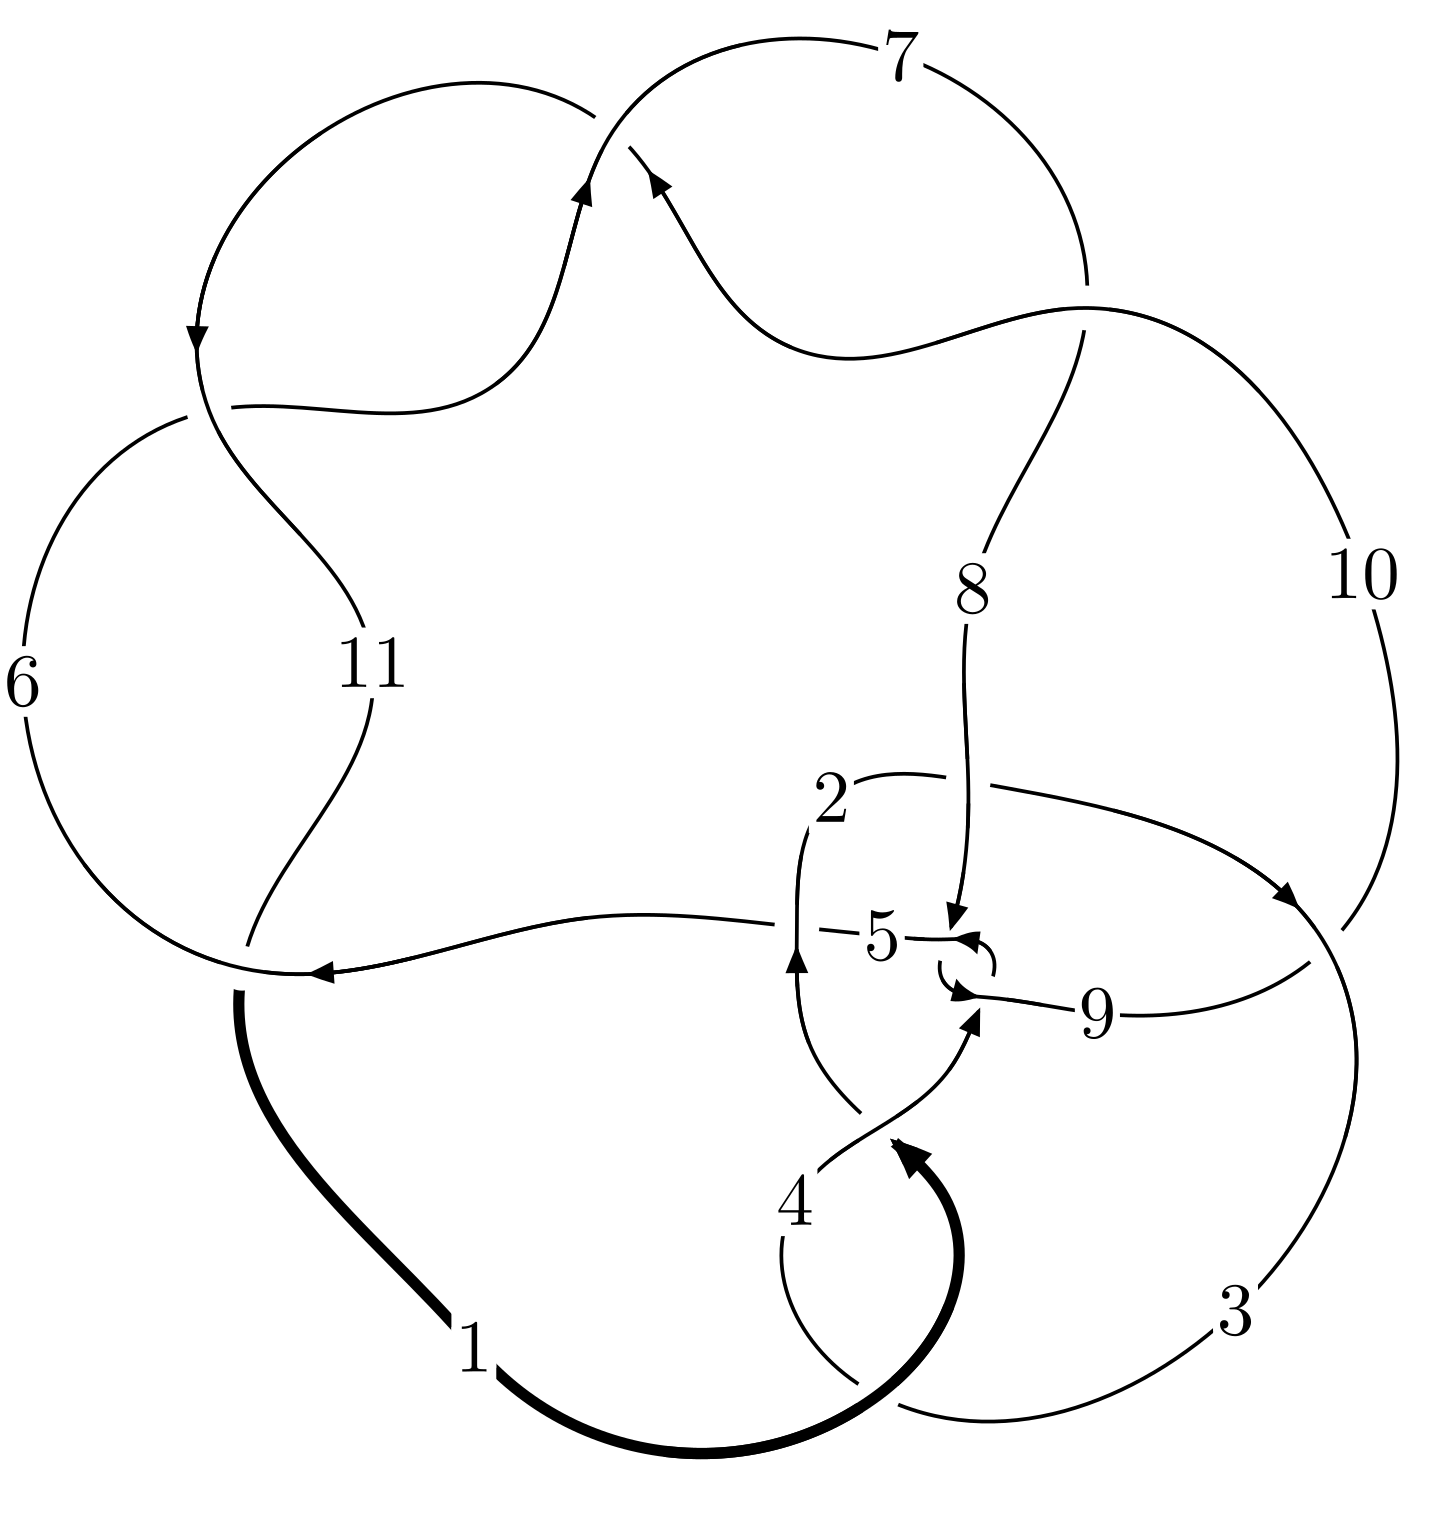
\includegraphics[width=112pt]{../../../GIT/diagram.site/Diagrams/png/548_11a_299.png}\\
\ \ \ A knot diagram\footnotemark}&
\allowdisplaybreaks
\textbf{Linearized knot diagam} \\
\cline{2-2}
 &
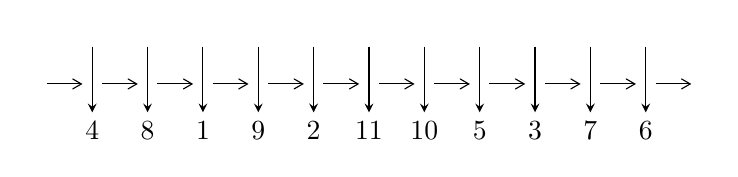
\begin{tikzpicture}[x=20pt, y=17pt]
	% nodes
	\node (C0) at (0, 0) {};
	\node (C1) at (1, 0) {};
	\node (C1U) at (1, +1) {};
	\node (C1D) at (1, -1) {4};

	\node (C2) at (2, 0) {};
	\node (C2U) at (2, +1) {};
	\node (C2D) at (2, -1) {8};

	\node (C3) at (3, 0) {};
	\node (C3U) at (3, +1) {};
	\node (C3D) at (3, -1) {1};

	\node (C4) at (4, 0) {};
	\node (C4U) at (4, +1) {};
	\node (C4D) at (4, -1) {9};

	\node (C5) at (5, 0) {};
	\node (C5U) at (5, +1) {};
	\node (C5D) at (5, -1) {2};

	\node (C6) at (6, 0) {};
	\node (C6U) at (6, +1) {};
	\node (C6D) at (6, -1) {11};

	\node (C7) at (7, 0) {};
	\node (C7U) at (7, +1) {};
	\node (C7D) at (7, -1) {10};

	\node (C8) at (8, 0) {};
	\node (C8U) at (8, +1) {};
	\node (C8D) at (8, -1) {5};

	\node (C9) at (9, 0) {};
	\node (C9U) at (9, +1) {};
	\node (C9D) at (9, -1) {3};

	\node (C10) at (10, 0) {};
	\node (C10U) at (10, +1) {};
	\node (C10D) at (10, -1) {7};

	\node (C11) at (11, 0) {};
	\node (C11U) at (11, +1) {};
	\node (C11D) at (11, -1) {6};
	\node (C12) at (12, 0) {};

	% arrows
	\draw[->,>={angle 60}]
	(C0) edge (C1) (C1) edge (C2) (C2) edge (C3) (C3) edge (C4) (C4) edge (C5) (C5) edge (C6) (C6) edge (C7) (C7) edge (C8) (C8) edge (C9) (C9) edge (C10) (C10) edge (C11) (C11) edge (C12) ;	\draw[->,>=stealth]
	(C1U) edge (C1D) (C2U) edge (C2D) (C3U) edge (C3D) (C4U) edge (C4D) (C5U) edge (C5D) (C6U) edge (C6D) (C7U) edge (C7D) (C8U) edge (C8D) (C9U) edge (C9D) (C10U) edge (C10D) (C11U) edge (C11D) ;
	\end{tikzpicture} \\
\hhline{~~} \\& 
\textbf{Solving Sequence} \\ \cline{2-2} 
 &
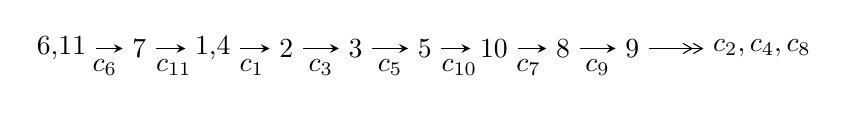
\begin{tikzpicture}[x=25pt, y=7pt]
	% node
	\node (A0) at (-1/8, 0) {6,11};
	\node (A1) at (1, 0) {7};
	\node (A2) at (33/16, 0) {1,4};
	\node (A3) at (25/8, 0) {2};
	\node (A4) at (33/8, 0) {3};
	\node (A5) at (41/8, 0) {5};
	\node (A6) at (49/8, 0) {10};
	\node (A7) at (57/8, 0) {8};
	\node (A8) at (65/8, 0) {9};
	\node (C1) at (1/2, -1) {$c_{6}$};
	\node (C2) at (3/2, -1) {$c_{11}$};
	\node (C3) at (21/8, -1) {$c_{1}$};
	\node (C4) at (29/8, -1) {$c_{3}$};
	\node (C5) at (37/8, -1) {$c_{5}$};
	\node (C6) at (45/8, -1) {$c_{10}$};
	\node (C7) at (53/8, -1) {$c_{7}$};
	\node (C8) at (61/8, -1) {$c_{9}$};
	\node (A9) at (10, 0) {$c_{2},c_{4},c_{8}$};

	% edge
	\draw[->,>=stealth]	
	(A0) edge (A1) (A1) edge (A2) (A2) edge (A3) (A3) edge (A4) (A4) edge (A5) (A5) edge (A6) (A6) edge (A7) (A7) edge (A8) ;
	\draw[->>,>={angle 60}]	
	(A8) edge (A9);
\end{tikzpicture} \\ 

\end{tabular} \\

\footnotetext{
The image of knot diagram is generated by the software ``\textbf{Draw programme}" developed by Andrew Bartholomew(\url{http://www.layer8.co.uk/maths/draw/index.htm\#Running-draw}), where we modified some parts for our purpose(\url{https://github.com/CATsTAILs/LinksPainter}).
}\phantom \\ \newline 
\centering \textbf{Ideals for irreducible components\footnotemark of $X_{\text{par}}$} 
 
\begin{align*}
I^u_{1}&=\langle 
-3.98094\times10^{27} u^{50}+3.57674\times10^{27} u^{49}+\cdots+5.12235\times10^{28} b-4.16694\times10^{28},\\
\phantom{I^u_{1}}&\phantom{= \langle  }4.56338\times10^{28} u^{50}+8.09970\times10^{28} u^{49}+\cdots+5.12235\times10^{28} a+2.57618\times10^{28},\;u^{51}+2 u^{50}+\cdots+u^2-1\rangle \\
I^u_{2}&=\langle 
u^2+5 b+3 u+4,\;4 u^2+5 a-8 u+6,\;u^3- u^2+2 u-1\rangle \\
\\
\end{align*}
\raggedright * 2 irreducible components of $\dim_{\mathbb{C}}=0$, with total 54 representations.\\
\footnotetext{All coefficients of polynomials are rational numbers. But the coefficients are sometimes approximated in decimal forms when there is not enough margin.}
\newpage
\renewcommand{\arraystretch}{1}
\centering \section*{I. $I^u_{1}= \langle -3.98\times10^{27} u^{50}+3.58\times10^{27} u^{49}+\cdots+5.12\times10^{28} b-4.17\times10^{28},\;4.56\times10^{28} u^{50}+8.10\times10^{28} u^{49}+\cdots+5.12\times10^{28} a+2.58\times10^{28},\;u^{51}+2 u^{50}+\cdots+u^2-1 \rangle$}
\flushleft \textbf{(i) Arc colorings}\\
\begin{tabular}{m{7pt} m{180pt} m{7pt} m{180pt} }
\flushright $a_{6}=$&$\begin{pmatrix}1\\0\end{pmatrix}$ \\
\flushright $a_{11}=$&$\begin{pmatrix}0\\u\end{pmatrix}$ \\
\flushright $a_{7}=$&$\begin{pmatrix}1\\u^2\end{pmatrix}$ \\
\flushright $a_{1}=$&$\begin{pmatrix}- u\\u\end{pmatrix}$ \\
\flushright $a_{4}=$&$\begin{pmatrix}-0.890878 u^{50}-1.58125 u^{49}+\cdots+2.76933 u-0.502929\\0.0777171 u^{50}-0.0698262 u^{49}+\cdots-0.830913 u+0.813483\end{pmatrix}$ \\
\flushright $a_{2}=$&$\begin{pmatrix}-0.911790 u^{50}-1.62215 u^{49}+\cdots+3.55461 u-0.444712\\0.00216816 u^{50}-0.149791 u^{49}+\cdots-0.143535 u+0.845107\end{pmatrix}$ \\
\flushright $a_{3}=$&$\begin{pmatrix}-0.848184 u^{50}-1.53135 u^{49}+\cdots+1.95617 u-0.527682\\0.0350226 u^{50}-0.119723 u^{49}+\cdots-0.0177518 u+0.838236\end{pmatrix}$ \\
\flushright $a_{5}=$&$\begin{pmatrix}0.219194 u^{50}+0.0575194 u^{49}+\cdots-2.71987 u+0.983462\\0.568042 u^{50}+1.43143 u^{49}+\cdots-0.564791 u+0.0862524\end{pmatrix}$ \\
\flushright $a_{10}=$&$\begin{pmatrix}u\\u^3+u\end{pmatrix}$ \\
\flushright $a_{8}=$&$\begin{pmatrix}u^2+1\\u^4+2 u^2\end{pmatrix}$ \\
\flushright $a_{9}=$&$\begin{pmatrix}1.21389 u^{50}+2.29120 u^{49}+\cdots-2.54183 u+0.639066\\-0.214736 u^{50}-0.901043 u^{49}+\cdots+1.59632 u+0.327975\end{pmatrix}$\\ \flushright $a_{9}=$&$\begin{pmatrix}1.21389 u^{50}+2.29120 u^{49}+\cdots-2.54183 u+0.639066\\-0.214736 u^{50}-0.901043 u^{49}+\cdots+1.59632 u+0.327975\end{pmatrix}$\\&\end{tabular}
\flushleft \textbf{(ii) Obstruction class $= -1$}\\~\\
\flushleft \textbf{(iii) Cusp Shapes $= 0.0485520 u^{50}-0.908190 u^{49}+\cdots-14.7258 u-8.93442$}\\~\\
\newpage\renewcommand{\arraystretch}{1}
\flushleft \textbf{(iv) u-Polynomials at the component}\newline \\
\begin{tabular}{m{50pt}|m{274pt}}
Crossings & \hspace{64pt}u-Polynomials at each crossing \\
\hline $$\begin{aligned}c_{1},c_{3}\end{aligned}$$&$\begin{aligned}
&u^{51}-4 u^{50}+\cdots-49 u+25
\end{aligned}$\\
\hline $$\begin{aligned}c_{2}\end{aligned}$$&$\begin{aligned}
&u^{51}+u^{50}+\cdots+380 u+200
\end{aligned}$\\
\hline $$\begin{aligned}c_{4},c_{8}\end{aligned}$$&$\begin{aligned}
&u^{51}+2 u^{50}+\cdots+4 u+1
\end{aligned}$\\
\hline $$\begin{aligned}c_{5}\end{aligned}$$&$\begin{aligned}
&5(5 u^{51}-28 u^{50}+\cdots-30 u+857)
\end{aligned}$\\
\hline $$\begin{aligned}c_{6},c_{7},c_{10}\\c_{11}\end{aligned}$$&$\begin{aligned}
&u^{51}-2 u^{50}+\cdots- u^2+1
\end{aligned}$\\
\hline $$\begin{aligned}c_{9}\end{aligned}$$&$\begin{aligned}
&5(5 u^{51}-9 u^{50}+\cdots+1703 u+239)
\end{aligned}$\\
\hline
\end{tabular}\\~\\
\newpage\renewcommand{\arraystretch}{1}
\flushleft \textbf{(v) Riley Polynomials at the component}\newline \\
\begin{tabular}{m{50pt}|m{274pt}}
Crossings & \hspace{64pt}Riley Polynomials at each crossing \\
\hline $$\begin{aligned}c_{1},c_{3}\end{aligned}$$&$\begin{aligned}
&y^{51}-26 y^{50}+\cdots+17851 y-625
\end{aligned}$\\
\hline $$\begin{aligned}c_{2}\end{aligned}$$&$\begin{aligned}
&y^{51}+21 y^{50}+\cdots-118000 y-40000
\end{aligned}$\\
\hline $$\begin{aligned}c_{4},c_{8}\end{aligned}$$&$\begin{aligned}
&y^{51}+28 y^{50}+\cdots+2 y-1
\end{aligned}$\\
\hline $$\begin{aligned}c_{5}\end{aligned}$$&$\begin{aligned}
&25(25 y^{51}+176 y^{50}+\cdots-1375442 y-734449)
\end{aligned}$\\
\hline $$\begin{aligned}c_{6},c_{7},c_{10}\\c_{11}\end{aligned}$$&$\begin{aligned}
&y^{51}+60 y^{50}+\cdots+2 y-1
\end{aligned}$\\
\hline $$\begin{aligned}c_{9}\end{aligned}$$&$\begin{aligned}
&25(25 y^{51}+739 y^{50}+\cdots-637947 y-57121)
\end{aligned}$\\
\hline
\end{tabular}\\~\\
\newpage\flushleft \textbf{(vi) Complex Volumes and Cusp Shapes}
$$\begin{array}{c|c|c}  
\text{Solutions to }I^u_{1}& \I (\text{vol} + \sqrt{-1}CS) & \text{Cusp shape}\\
 \hline 
\begin{aligned}
u &= -0.552527 + 0.820307 I \\
a &= \phantom{-}0.48391 - 1.52868 I \\
b &= -1.72817 + 0.85216 I\end{aligned}
 & \phantom{-}2.62483 + 11.59540 I & -7.79067 - 8.85645 I \\ \hline\begin{aligned}
u &= -0.552527 - 0.820307 I \\
a &= \phantom{-}0.48391 + 1.52868 I \\
b &= -1.72817 - 0.85216 I\end{aligned}
 & \phantom{-}2.62483 - 11.59540 I & -7.79067 + 8.85645 I \\ \hline\begin{aligned}
u &= \phantom{-}0.589306 + 0.788540 I \\
a &= -0.51919 - 1.38595 I \\
b &= \phantom{-}1.55822 + 0.77897 I\end{aligned}
 & -0.80955 - 5.70999 I & -10.32903 + 7.24097 I \\ \hline\begin{aligned}
u &= \phantom{-}0.589306 - 0.788540 I \\
a &= -0.51919 + 1.38595 I \\
b &= \phantom{-}1.55822 - 0.77897 I\end{aligned}
 & -0.80955 + 5.70999 I & -10.32903 - 7.24097 I \\ \hline\begin{aligned}
u &= -0.433100 + 0.988087 I \\
a &= \phantom{-}0.85921 - 1.15463 I \\
b &= -0.784864 + 0.164197 I\end{aligned}
 & \phantom{-}3.75291 - 3.24873 I & -11.00000 + 0. I\phantom{ +0.000000I} \\ \hline\begin{aligned}
u &= -0.433100 - 0.988087 I \\
a &= \phantom{-}0.85921 + 1.15463 I \\
b &= -0.784864 - 0.164197 I\end{aligned}
 & \phantom{-}3.75291 + 3.24873 I & -11.00000 + 0. I\phantom{ +0.000000I} \\ \hline\begin{aligned}
u &= -0.376973 + 0.809467 I \\
a &= \phantom{-}1.031830 - 0.475824 I \\
b &= -0.043546 - 0.349975 I\end{aligned}
 & \phantom{-}5.59371 + 5.41403 I & -4.14016 - 6.52359 I \\ \hline\begin{aligned}
u &= -0.376973 - 0.809467 I \\
a &= \phantom{-}1.031830 + 0.475824 I \\
b &= -0.043546 + 0.349975 I\end{aligned}
 & \phantom{-}5.59371 - 5.41403 I & -4.14016 + 6.52359 I \\ \hline\begin{aligned}
u &= \phantom{-}0.249787 + 0.812726 I \\
a &= -0.469781 - 0.492664 I \\
b &= -0.095865 + 0.184201 I\end{aligned}
 & \phantom{-}1.73380 - 1.81855 I & -6.35906 + 4.36354 I \\ \hline\begin{aligned}
u &= \phantom{-}0.249787 - 0.812726 I \\
a &= -0.469781 + 0.492664 I \\
b &= -0.095865 - 0.184201 I\end{aligned}
 & \phantom{-}1.73380 + 1.81855 I & -6.35906 - 4.36354 I\\
 \hline 
 \end{array}$$\newpage$$\begin{array}{c|c|c}  
\text{Solutions to }I^u_{1}& \I (\text{vol} + \sqrt{-1}CS) & \text{Cusp shape}\\
 \hline 
\begin{aligned}
u &= -0.493565 + 0.692270 I \\
a &= \phantom{-}0.247144 - 1.224100 I \\
b &= -1.21189 + 1.00104 I\end{aligned}
 & \phantom{-}4.68147 + 1.04951 I & -4.16172 - 4.32794 I \\ \hline\begin{aligned}
u &= -0.493565 - 0.692270 I \\
a &= \phantom{-}0.247144 + 1.224100 I \\
b &= -1.21189 - 1.00104 I\end{aligned}
 & \phantom{-}4.68147 - 1.04951 I & -4.16172 + 4.32794 I \\ \hline\begin{aligned}
u &= \phantom{-}0.773905 + 0.191317 I \\
a &= -0.320071 - 0.624747 I \\
b &= \phantom{-}1.381640 - 0.030498 I\end{aligned}
 & -2.64708 + 1.15805 I & -10.73331 - 5.02870 I \\ \hline\begin{aligned}
u &= \phantom{-}0.773905 - 0.191317 I \\
a &= -0.320071 + 0.624747 I \\
b &= \phantom{-}1.381640 + 0.030498 I\end{aligned}
 & -2.64708 - 1.15805 I & -10.73331 + 5.02870 I \\ \hline\begin{aligned}
u &= -0.744224 + 0.089987 I \\
a &= \phantom{-}0.047354 - 0.638462 I \\
b &= -1.47794 - 0.27354 I\end{aligned}
 & \phantom{-}0.42114 - 7.27131 I & -10.81656 + 5.67006 I \\ \hline\begin{aligned}
u &= -0.744224 - 0.089987 I \\
a &= \phantom{-}0.047354 + 0.638462 I \\
b &= -1.47794 + 0.27354 I\end{aligned}
 & \phantom{-}0.42114 + 7.27131 I & -10.81656 - 5.67006 I \\ \hline\begin{aligned}
u &= \phantom{-}0.128736 + 0.681128 I \\
a &= \phantom{-}1.63090 - 0.76962 I \\
b &= -1.72989 + 2.00427 I\end{aligned}
 & \phantom{-}1.377800 + 0.247335 I & -11.41702 + 6.59841 I \\ \hline\begin{aligned}
u &= \phantom{-}0.128736 - 0.681128 I \\
a &= \phantom{-}1.63090 + 0.76962 I \\
b &= -1.72989 - 2.00427 I\end{aligned}
 & \phantom{-}1.377800 - 0.247335 I & -11.41702 - 6.59841 I \\ \hline\begin{aligned}
u &= \phantom{-}0.328726 + 0.602476 I \\
a &= -0.683354 + 0.933926 I \\
b &= -1.027660 - 0.198210 I\end{aligned}
 & \phantom{-}0.09032 - 4.00238 I & -9.47119 + 9.47766 I \\ \hline\begin{aligned}
u &= \phantom{-}0.328726 - 0.602476 I \\
a &= -0.683354 - 0.933926 I \\
b &= -1.027660 + 0.198210 I\end{aligned}
 & \phantom{-}0.09032 + 4.00238 I & -9.47119 - 9.47766 I\\
 \hline 
 \end{array}$$\newpage$$\begin{array}{c|c|c}  
\text{Solutions to }I^u_{1}& \I (\text{vol} + \sqrt{-1}CS) & \text{Cusp shape}\\
 \hline 
\begin{aligned}
u &= \phantom{-}0.309159 + 1.281950 I \\
a &= -0.53813 - 1.48328 I \\
b &= \phantom{-}0.630951 + 0.896457 I\end{aligned}
 & \phantom{-}1.88408 - 2.74356 I & \phantom{-0.000000 } 0 \\ \hline\begin{aligned}
u &= \phantom{-}0.309159 - 1.281950 I \\
a &= -0.53813 + 1.48328 I \\
b &= \phantom{-}0.630951 - 0.896457 I\end{aligned}
 & \phantom{-}1.88408 + 2.74356 I & \phantom{-0.000000 } 0 \\ \hline\begin{aligned}
u &= -0.235448 + 0.507844 I \\
a &= \phantom{-}0.06586 + 1.89337 I \\
b &= \phantom{-}1.226960 - 0.240501 I\end{aligned}
 & -1.46138 + 0.98661 I & -12.15795 - 1.22039 I \\ \hline\begin{aligned}
u &= -0.235448 - 0.507844 I \\
a &= \phantom{-}0.06586 - 1.89337 I \\
b &= \phantom{-}1.226960 + 0.240501 I\end{aligned}
 & -1.46138 - 0.98661 I & -12.15795 + 1.22039 I \\ \hline\begin{aligned}
u &= -0.535402 + 0.073202 I \\
a &= \phantom{-}0.434598 - 1.044040 I \\
b &= -0.708461 - 0.403158 I\end{aligned}
 & \phantom{-}3.00953 + 2.35838 I & -8.15249 - 2.65728 I \\ \hline\begin{aligned}
u &= -0.535402 - 0.073202 I \\
a &= \phantom{-}0.434598 + 1.044040 I \\
b &= -0.708461 + 0.403158 I\end{aligned}
 & \phantom{-}3.00953 - 2.35838 I & -8.15249 + 2.65728 I \\ \hline\begin{aligned}
u &= -0.271262 + 0.396700 I \\
a &= \phantom{-}0.75415 + 2.38170 I \\
b &= \phantom{-}0.944727 - 0.152860 I\end{aligned}
 & -1.67074 + 1.07820 I & -12.01082 - 5.84608 I \\ \hline\begin{aligned}
u &= -0.271262 - 0.396700 I \\
a &= \phantom{-}0.75415 - 2.38170 I \\
b &= \phantom{-}0.944727 + 0.152860 I\end{aligned}
 & -1.67074 - 1.07820 I & -12.01082 + 5.84608 I \\ \hline\begin{aligned}
u &= -0.01718 + 1.55667 I \\
a &= -0.37477 + 2.03786 I \\
b &= \phantom{-}0.552519 - 1.004140 I\end{aligned}
 & \phantom{-}5.04838 + 1.69001 I & \phantom{-0.000000 } 0 \\ \hline\begin{aligned}
u &= -0.01718 - 1.55667 I \\
a &= -0.37477 - 2.03786 I \\
b &= \phantom{-}0.552519 + 1.004140 I\end{aligned}
 & \phantom{-}5.04838 - 1.69001 I & \phantom{-0.000000 } 0\\
 \hline 
 \end{array}$$\newpage$$\begin{array}{c|c|c}  
\text{Solutions to }I^u_{1}& \I (\text{vol} + \sqrt{-1}CS) & \text{Cusp shape}\\
 \hline 
\begin{aligned}
u &= -0.04180 + 1.57969 I \\
a &= -1.09580 + 1.51782 I \\
b &= \phantom{-}1.49270 - 0.77222 I\end{aligned}
 & \phantom{-}5.80181 + 1.83329 I & \phantom{-0.000000 } 0 \\ \hline\begin{aligned}
u &= -0.04180 - 1.57969 I \\
a &= -1.09580 - 1.51782 I \\
b &= \phantom{-}1.49270 + 0.77222 I\end{aligned}
 & \phantom{-}5.80181 - 1.83329 I & \phantom{-0.000000 } 0 \\ \hline\begin{aligned}
u &= \phantom{-}0.06969 + 1.58540 I \\
a &= \phantom{-}0.646529 + 0.973357 I \\
b &= -1.354660 - 0.387992 I\end{aligned}
 & \phantom{-}7.57583 - 5.34940 I & \phantom{-0.000000 } 0 \\ \hline\begin{aligned}
u &= \phantom{-}0.06969 - 1.58540 I \\
a &= \phantom{-}0.646529 - 0.973357 I \\
b &= -1.354660 + 0.387992 I\end{aligned}
 & \phantom{-}7.57583 + 5.34940 I & \phantom{-0.000000 } 0 \\ \hline\begin{aligned}
u &= \phantom{-}0.339596 + 0.188204 I \\
a &= -1.55128 + 2.09918 I \\
b &= -0.402028 + 0.283631 I\end{aligned}
 & -1.01423 + 1.50344 I & -14.02114 - 0.26378 I \\ \hline\begin{aligned}
u &= \phantom{-}0.339596 - 0.188204 I \\
a &= -1.55128 - 2.09918 I \\
b &= -0.402028 - 0.283631 I\end{aligned}
 & -1.01423 - 1.50344 I & -14.02114 + 0.26378 I \\ \hline\begin{aligned}
u &= \phantom{-}0.02693 + 1.61334 I \\
a &= \phantom{-}3.90639 - 0.28673 I \\
b &= -3.98695 + 0.78800 I\end{aligned}
 & \phantom{-}9.33157 - 0.28182 I & \phantom{-0.000000 } 0 \\ \hline\begin{aligned}
u &= \phantom{-}0.02693 - 1.61334 I \\
a &= \phantom{-}3.90639 + 0.28673 I \\
b &= -3.98695 - 0.78800 I\end{aligned}
 & \phantom{-}9.33157 + 0.28182 I & \phantom{-0.000000 } 0 \\ \hline\begin{aligned}
u &= -0.15866 + 1.61313 I \\
a &= \phantom{-}0.90457 - 2.22903 I \\
b &= -1.33704 + 1.71038 I\end{aligned}
 & \phantom{-}12.51670 + 3.55318 I & \phantom{-0.000000 } 0 \\ \hline\begin{aligned}
u &= -0.15866 - 1.61313 I \\
a &= \phantom{-}0.90457 + 2.22903 I \\
b &= -1.33704 - 1.71038 I\end{aligned}
 & \phantom{-}12.51670 - 3.55318 I & \phantom{-0.000000 } 0\\
 \hline 
 \end{array}$$\newpage$$\begin{array}{c|c|c}  
\text{Solutions to }I^u_{1}& \I (\text{vol} + \sqrt{-1}CS) & \text{Cusp shape}\\
 \hline 
\begin{aligned}
u &= -0.10468 + 1.64228 I \\
a &= \phantom{-}0.285194 + 0.100077 I \\
b &= \phantom{-}0.495111 - 0.386510 I\end{aligned}
 & \phantom{-}14.0417 + 7.2484 I & \phantom{-0.000000 } 0 \\ \hline\begin{aligned}
u &= -0.10468 - 1.64228 I \\
a &= \phantom{-}0.285194 - 0.100077 I \\
b &= \phantom{-}0.495111 + 0.386510 I\end{aligned}
 & \phantom{-}14.0417 - 7.2484 I & \phantom{-0.000000 } 0 \\ \hline\begin{aligned}
u &= \phantom{-}0.08123 + 1.64771 I \\
a &= \phantom{-}0.021744 - 0.179863 I \\
b &= -0.560164 + 0.015522 I\end{aligned}
 & \phantom{-}10.29890 - 3.16367 I & \phantom{-0.000000 } 0 \\ \hline\begin{aligned}
u &= \phantom{-}0.08123 - 1.64771 I \\
a &= \phantom{-}0.021744 + 0.179863 I \\
b &= -0.560164 - 0.015522 I\end{aligned}
 & \phantom{-}10.29890 + 3.16367 I & \phantom{-0.000000 } 0 \\ \hline\begin{aligned}
u &= \phantom{-}0.17216 + 1.64138 I \\
a &= -1.15226 - 2.05629 I \\
b &= \phantom{-}1.58595 + 1.37531 I\end{aligned}
 & \phantom{-}7.44997 - 8.60283 I & \phantom{-0.000000 } 0 \\ \hline\begin{aligned}
u &= \phantom{-}0.17216 - 1.64138 I \\
a &= -1.15226 + 2.05629 I \\
b &= \phantom{-}1.58595 - 1.37531 I\end{aligned}
 & \phantom{-}7.44997 + 8.60283 I & \phantom{-0.000000 } 0 \\ \hline\begin{aligned}
u &= -0.16225 + 1.65033 I \\
a &= \phantom{-}1.31880 - 2.12033 I \\
b &= -1.83667 + 1.38127 I\end{aligned}
 & \phantom{-}11.0558 + 14.3418 I & \phantom{-0.000000 } 0 \\ \hline\begin{aligned}
u &= -0.16225 - 1.65033 I \\
a &= \phantom{-}1.31880 + 2.12033 I \\
b &= -1.83667 - 1.38127 I\end{aligned}
 & \phantom{-}11.0558 - 14.3418 I & \phantom{-0.000000 } 0 \\ \hline\begin{aligned}
u &= -0.08999 + 1.68712 I \\
a &= \phantom{-}0.334351 - 0.580821 I \\
b &= \phantom{-}0.022884 + 0.143685 I\end{aligned}
 & \phantom{-}13.10850 - 1.33730 I & \phantom{-0.000000 } 0 \\ \hline\begin{aligned}
u &= -0.08999 - 1.68712 I \\
a &= \phantom{-}0.334351 + 0.580821 I \\
b &= \phantom{-}0.022884 - 0.143685 I\end{aligned}
 & \phantom{-}13.10850 + 1.33730 I & \phantom{-0.000000 } 0\\
 \hline 
 \end{array}$$\newpage$$\begin{array}{c|c|c}  
\text{Solutions to }I^u_{1}& \I (\text{vol} + \sqrt{-1}CS) & \text{Cusp shape}\\
 \hline 
\begin{aligned}
u &= \phantom{-}0.295696\phantom{ +0.000000I} \\
a &= -0.935819\phantom{ +0.000000I} \\
b &= \phantom{-}0.188257\phantom{ +0.000000I}\end{aligned}
 & -0.590385\phantom{ +0.000000I} & -17.0960\phantom{ +0.000000I}\\
 \hline 
 \end{array}$$\newpage\newpage\renewcommand{\arraystretch}{1}
\centering \section*{II. $I^u_{2}= \langle u^2+5 b+3 u+4,\;4 u^2+5 a-8 u+6,\;u^3- u^2+2 u-1 \rangle$}
\flushleft \textbf{(i) Arc colorings}\\
\begin{tabular}{m{7pt} m{180pt} m{7pt} m{180pt} }
\flushright $a_{6}=$&$\begin{pmatrix}1\\0\end{pmatrix}$ \\
\flushright $a_{11}=$&$\begin{pmatrix}0\\u\end{pmatrix}$ \\
\flushright $a_{7}=$&$\begin{pmatrix}1\\u^2\end{pmatrix}$ \\
\flushright $a_{1}=$&$\begin{pmatrix}- u\\u\end{pmatrix}$ \\
\flushright $a_{4}=$&$\begin{pmatrix}-\frac{4}{5} u^2+\frac{8}{5} u-\frac{6}{5}\\-\frac{1}{5} u^2-\frac{3}{5} u-\frac{4}{5}\end{pmatrix}$ \\
\flushright $a_{2}=$&$\begin{pmatrix}-\frac{4}{5} u^2+\frac{3}{5} u-\frac{6}{5}\\-\frac{1}{5} u^2+\frac{2}{5} u-\frac{4}{5}\end{pmatrix}$ \\
\flushright $a_{3}=$&$\begin{pmatrix}-\frac{4}{5} u^2+\frac{3}{5} u-\frac{6}{5}\\-\frac{1}{5} u^2+\frac{2}{5} u-\frac{4}{5}\end{pmatrix}$ \\
\flushright $a_{5}=$&$\begin{pmatrix}-\frac{13}{25} u^2+\frac{6}{25} u+\frac{8}{25}\\-\frac{7}{25} u^2+\frac{9}{25} u-\frac{13}{25}\end{pmatrix}$ \\
\flushright $a_{10}=$&$\begin{pmatrix}u\\u^2- u+1\end{pmatrix}$ \\
\flushright $a_{8}=$&$\begin{pmatrix}u^2+1\\u^2- u+1\end{pmatrix}$ \\
\flushright $a_{9}=$&$\begin{pmatrix}\frac{4}{25} u^2+\frac{27}{25} u+\frac{11}{25}\\\frac{31}{25} u^2-\frac{22}{25} u+\frac{29}{25}\end{pmatrix}$\\ \flushright $a_{9}=$&$\begin{pmatrix}\frac{4}{25} u^2+\frac{27}{25} u+\frac{11}{25}\\\frac{31}{25} u^2-\frac{22}{25} u+\frac{29}{25}\end{pmatrix}$\\&\end{tabular}
\flushleft \textbf{(ii) Obstruction class $= 1$}\\~\\
\flushleft \textbf{(iii) Cusp Shapes $= -\frac{12}{25} u^2+\frac{69}{25} u-\frac{408}{25}$}\\~\\
\newpage\renewcommand{\arraystretch}{1}
\flushleft \textbf{(iv) u-Polynomials at the component}\newline \\
\begin{tabular}{m{50pt}|m{274pt}}
Crossings & \hspace{64pt}u-Polynomials at each crossing \\
\hline $$\begin{aligned}c_{1}\end{aligned}$$&$\begin{aligned}
&(u-1)^3
\end{aligned}$\\
\hline $$\begin{aligned}c_{2}\end{aligned}$$&$\begin{aligned}
&u^3
\end{aligned}$\\
\hline $$\begin{aligned}c_{3}\end{aligned}$$&$\begin{aligned}
&(u+1)^3
\end{aligned}$\\
\hline $$\begin{aligned}c_{4}\end{aligned}$$&$\begin{aligned}
&u^3+u^2-1
\end{aligned}$\\
\hline $$\begin{aligned}c_{5}\end{aligned}$$&$\begin{aligned}
&5(5 u^3+7 u^2+4 u+1)
\end{aligned}$\\
\hline $$\begin{aligned}c_{6},c_{7}\end{aligned}$$&$\begin{aligned}
&u^3- u^2+2 u-1
\end{aligned}$\\
\hline $$\begin{aligned}c_{8}\end{aligned}$$&$\begin{aligned}
&u^3- u^2+1
\end{aligned}$\\
\hline $$\begin{aligned}c_{9}\end{aligned}$$&$\begin{aligned}
&5(5 u^3+4 u^2- u-1)
\end{aligned}$\\
\hline $$\begin{aligned}c_{10},c_{11}\end{aligned}$$&$\begin{aligned}
&u^3+u^2+2 u+1
\end{aligned}$\\
\hline
\end{tabular}\\~\\
\newpage\renewcommand{\arraystretch}{1}
\flushleft \textbf{(v) Riley Polynomials at the component}\newline \\
\begin{tabular}{m{50pt}|m{274pt}}
Crossings & \hspace{64pt}Riley Polynomials at each crossing \\
\hline $$\begin{aligned}c_{1},c_{3}\end{aligned}$$&$\begin{aligned}
&(y-1)^3
\end{aligned}$\\
\hline $$\begin{aligned}c_{2}\end{aligned}$$&$\begin{aligned}
&y^3
\end{aligned}$\\
\hline $$\begin{aligned}c_{4},c_{8}\end{aligned}$$&$\begin{aligned}
&y^3- y^2+2 y-1
\end{aligned}$\\
\hline $$\begin{aligned}c_{5}\end{aligned}$$&$\begin{aligned}
&25(25 y^3-9 y^2+2 y-1)
\end{aligned}$\\
\hline $$\begin{aligned}c_{6},c_{7},c_{10}\\c_{11}\end{aligned}$$&$\begin{aligned}
&y^3+3 y^2+2 y-1
\end{aligned}$\\
\hline $$\begin{aligned}c_{9}\end{aligned}$$&$\begin{aligned}
&25(25 y^3-26 y^2+9 y-1)
\end{aligned}$\\
\hline
\end{tabular}\\~\\
\newpage\flushleft \textbf{(vi) Complex Volumes and Cusp Shapes}
$$\begin{array}{c|c|c}  
\text{Solutions to }I^u_{2}& \I (\text{vol} + \sqrt{-1}CS) & \text{Cusp shape}\\
 \hline 
\begin{aligned}
u &= \phantom{-}0.215080 + 1.307140 I \\
a &= \phantom{-}0.47401 + 1.64160 I \\
b &= -0.596576 - 0.896741 I\end{aligned}
 & \phantom{-}1.37919 - 2.82812 I & -14.9284 + 3.3378 I \\ \hline\begin{aligned}
u &= \phantom{-}0.215080 - 1.307140 I \\
a &= \phantom{-}0.47401 - 1.64160 I \\
b &= -0.596576 + 0.896741 I\end{aligned}
 & \phantom{-}1.37919 + 2.82812 I & -14.9284 - 3.3378 I \\ \hline\begin{aligned}
u &= \phantom{-}0.569840\phantom{ +0.000000I} \\
a &= -0.548030\phantom{ +0.000000I} \\
b &= -1.20685\phantom{ +0.000000I}\end{aligned}
 & -2.75839\phantom{ +0.000000I} & -14.9030\phantom{ +0.000000I}\\
 \hline 
 \end{array}$$\newpage
\newpage\renewcommand{\arraystretch}{1}
\centering \section*{ III. u-Polynomials}
\begin{tabular}{m{50pt}|m{274pt}}
Crossings & \hspace{64pt}u-Polynomials at each crossing \\
\hline $$\begin{aligned}c_{1}\end{aligned}$$&$\begin{aligned}
&((u-1)^3)(u^{51}-4 u^{50}+\cdots-49 u+25)
\end{aligned}$\\
\hline $$\begin{aligned}c_{2}\end{aligned}$$&$\begin{aligned}
&u^3(u^{51}+u^{50}+\cdots+380 u+200)
\end{aligned}$\\
\hline $$\begin{aligned}c_{3}\end{aligned}$$&$\begin{aligned}
&((u+1)^3)(u^{51}-4 u^{50}+\cdots-49 u+25)
\end{aligned}$\\
\hline $$\begin{aligned}c_{4}\end{aligned}$$&$\begin{aligned}
&(u^3+u^2-1)(u^{51}+2 u^{50}+\cdots+4 u+1)
\end{aligned}$\\
\hline $$\begin{aligned}c_{5}\end{aligned}$$&$\begin{aligned}
&25(5 u^3+7 u^2+4 u+1)(5 u^{51}-28 u^{50}+\cdots-30 u+857)
\end{aligned}$\\
\hline $$\begin{aligned}c_{6},c_{7}\end{aligned}$$&$\begin{aligned}
&(u^3- u^2+2 u-1)(u^{51}-2 u^{50}+\cdots- u^2+1)
\end{aligned}$\\
\hline $$\begin{aligned}c_{8}\end{aligned}$$&$\begin{aligned}
&(u^3- u^2+1)(u^{51}+2 u^{50}+\cdots+4 u+1)
\end{aligned}$\\
\hline $$\begin{aligned}c_{9}\end{aligned}$$&$\begin{aligned}
&25(5 u^3+4 u^2- u-1)(5 u^{51}-9 u^{50}+\cdots+1703 u+239)
\end{aligned}$\\
\hline $$\begin{aligned}c_{10},c_{11}\end{aligned}$$&$\begin{aligned}
&(u^3+u^2+2 u+1)(u^{51}-2 u^{50}+\cdots- u^2+1)
\end{aligned}$\\
\hline
\end{tabular}\newpage\renewcommand{\arraystretch}{1}
\centering \section*{ IV. Riley Polynomials}
\begin{tabular}{m{50pt}|m{274pt}}
Crossings & \hspace{64pt}Riley Polynomials at each crossing \\
\hline $$\begin{aligned}c_{1},c_{3}\end{aligned}$$&$\begin{aligned}
&((y-1)^3)(y^{51}-26 y^{50}+\cdots+17851 y-625)
\end{aligned}$\\
\hline $$\begin{aligned}c_{2}\end{aligned}$$&$\begin{aligned}
&y^3(y^{51}+21 y^{50}+\cdots-118000 y-40000)
\end{aligned}$\\
\hline $$\begin{aligned}c_{4},c_{8}\end{aligned}$$&$\begin{aligned}
&(y^3- y^2+2 y-1)(y^{51}+28 y^{50}+\cdots+2 y-1)
\end{aligned}$\\
\hline $$\begin{aligned}c_{5}\end{aligned}$$&$\begin{aligned}
&625(25 y^3-9 y^2+2 y-1)\\
&\cdot(25 y^{51}+176 y^{50}+\cdots-1375442 y-734449)
\end{aligned}$\\
\hline $$\begin{aligned}c_{6},c_{7},c_{10}\\c_{11}\end{aligned}$$&$\begin{aligned}
&(y^3+3 y^2+2 y-1)(y^{51}+60 y^{50}+\cdots+2 y-1)
\end{aligned}$\\
\hline $$\begin{aligned}c_{9}\end{aligned}$$&$\begin{aligned}
&625(25 y^3-26 y^2+9 y-1)(25 y^{51}+739 y^{50}+\cdots-637947 y-57121)
\end{aligned}$\\
\hline
\end{tabular}
\vskip 2pc
\end{document}